
\section{Question 1}
\label{part1}

\begin{itemize}
\item Using the pages from A3 that boilerpipe successfully processed, download those representations again \& reprocess them with boilerpipe.:
\item Document the time difference (e.g., Time(A4) – Time(A3)).
\item Compute the Jaccard Distance x for each pair of pages (i.e., P(A3) \& P(A4) for:
 \begin{itemize}
\item Unique terms (i.e., unigrams)
\item Bigrams
\item Trigrams
\end{itemize}
\item See:\url{http://en.wikipedia.org/wiki/Jaccard_index }
\item For each of the 3 cases (i.e., 1-, 2-, 3-grams) build a Cumulative Distribution Function that shows the \% change on the x-axis \& the \% of the population on the x-axis
\item See:\url {http://en.wikipedia.org/wiki/Cumulative_distribution_function}
\item Give 3-4 examples illustrating the range of change that you have measured.
\end{itemize}
\subsection{Solution}

\begin{itemize}
	\item I used the same script `getText.py' from A3 which uses `jusText'\cite{jusText} to remove templates from HTML files of 10000 URIs.
	\item `jusText'\cite{jusText} is a tool for removing boilerplate content such as navigation links, headers and footers from HTML pages.
	\item The time difference between processing boilerpipe of A3 and A4 was 27 days.
\end{itemize}

 \subsection{Code Listing}
Here is the python code that generate n-grams and computes Jaccard Distance.
\lstinputlisting[language=Python,breaklines = true,frame=single,caption={Python program to find unigrams, bigrams, trigrams}, label=lst:q1-1,captionpos=b,numbers=left,showspaces=false,showstringspaces=false,basicstyle=\footnotesize]{getNgrams.py}
\newpage 
I referred to a sample of code that constructs CDF from r-bloggers\cite{Cumulative} website.

Here is the R code which plots CDF for unigrams,bigrams,trigrams.
\lstinputlisting[breaklines = true,frame=single,caption={R program to plot unigrams, bigrams, trigrams change}, label=lst:q1-1,captionpos=b,numbers=left,showspaces=false,showstringspaces=false,basicstyle=\footnotesize]{unigramCD.R}

\begin{figure}[ht]
	\begin{center}
		 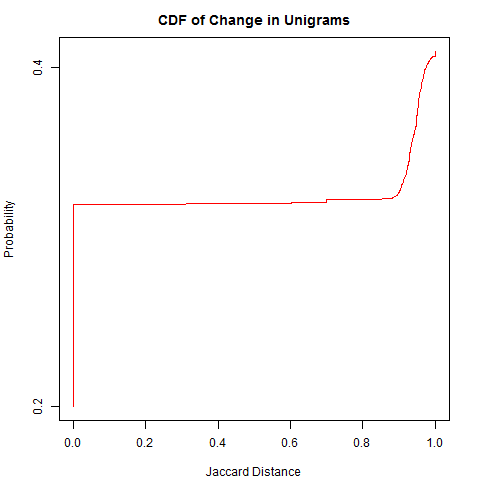
\includegraphics[scale=0.60]{Unigramq1}
		  \caption{CDF of change in unigrams}
	 \end{center}
\end{figure}
\begin{figure}[ht]
	\begin{center}
		 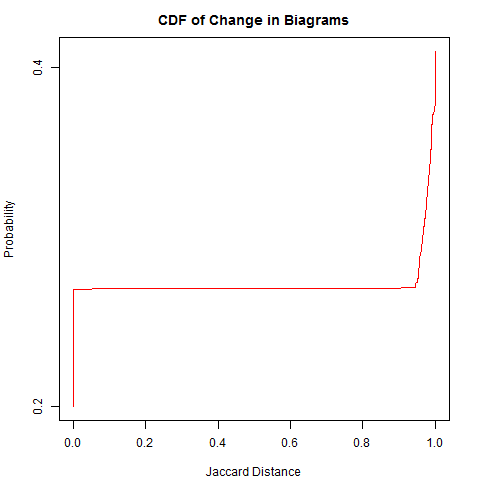
\includegraphics[scale=0.60]{bigramsq1}
		  \caption{CDF of change in bigrams}
	 \end{center}
\end{figure}
\newpage
\begin{figure}[ht]
	\begin{center}
		 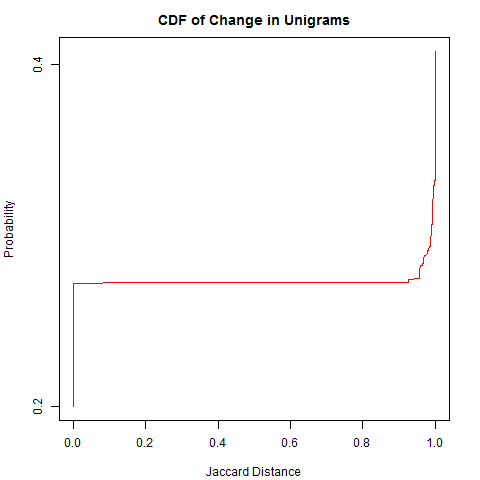
\includegraphics[scale=0.60]{Trigramq1}
		  \caption{CDF of change in trigrams}
	 \end{center}
\end{figure}
\newpage
\subsection{Examples}
Below are 3 examples with data that shows range of change.

\begin{itemize}
\item \url{http://www.foxnews.com/us/2015/02/09/judge-rules-utah-woman-accused-leaving-baby-in-trash-is-incompetent-to-stand/?cmpid=cmty_twitter_fn}\\
\begin{tabular}{|c|c|c|}
    \hline
    Unigrams & Bigrams & Trigrams\\
    \hline
    0.971 & 0.700 & 0.789\\
    \hline
\end{tabular}

\item \url{http://www.ebay.com/itm/like/301515875453?item=301515875453&lgeo=1&utm_medium=twitter&utm_source=dlvr.it&vectorid=229466&rmvSB=true}\\
\begin{tabular}{|c|c|c|}
    \hline
    Unigrams & Bigrams & Trigrams\\
    \hline
    0.471 & 0.600 & 0.689\\
    \hline
\end{tabular}

\item  
\url{http://du3a.org}\\
\begin{tabular}{|c|c|c|}
    \hline
    Unigrams & Bigrams & Trigrams\\
    \hline
    0.771 & 0.890 & 0.880\\
    \hline
\end{tabular}
\end{itemize}




